\documentclass[9pt]{IEEEtran}

\usepackage[english]{babel}
\usepackage{graphicx}
\usepackage{epstopdf}
\usepackage{fancyhdr}
\usepackage{amsmath}
\usepackage{amsthm}
\usepackage{amssymb}
\usepackage{url}
\usepackage{array}
\usepackage{textcomp}
\usepackage{listings}
\usepackage{hyperref}
\usepackage{xcolor}
\usepackage{colortbl}
\usepackage{float}
\usepackage{gensymb}
\usepackage{longtable}
\usepackage{supertabular}
\usepackage{multicol}

\usepackage[utf8x]{inputenc}

\usepackage[T1]{fontenc}
\usepackage{lmodern}
\input{glyphtounicode}
\pdfgentounicode=1

\graphicspath{{./figures/}}
\DeclareGraphicsExtensions{.pdf,.png,.jpg,.eps}

% correct bad hyphenation here
\hyphenation{op-tical net-works semi-conduc-tor trig-gs}

% ============================================================================================

\title{\vspace{0ex}
Programming part}


% ============================================================================================

\begin{document}

\maketitle

\section{Problem 5}
\subsection{Closest point projection implementation}
Firstly, to be able to use Projected Gradient Descent (PGD), we needed to implement projections onto the domains of interest. We implemented projections onto three different domains, as follows:

\begin{itemize}
    \item A circle with center at \((0,0)\) and radius \(\sqrt{1.5}\)
    \item A square: \([-2, 2] \times [-2, 2]\)
    \item A triangle with vertices \((-1, -1)\), \((1.5, -1)\), and \((-1, 1.5)\)
\end{itemize}


Figure~\ref{fig:proj} shows the projections of various points onto these domains. 
\vspace{-0pt}
\begin{figure}[h]
    \centering
    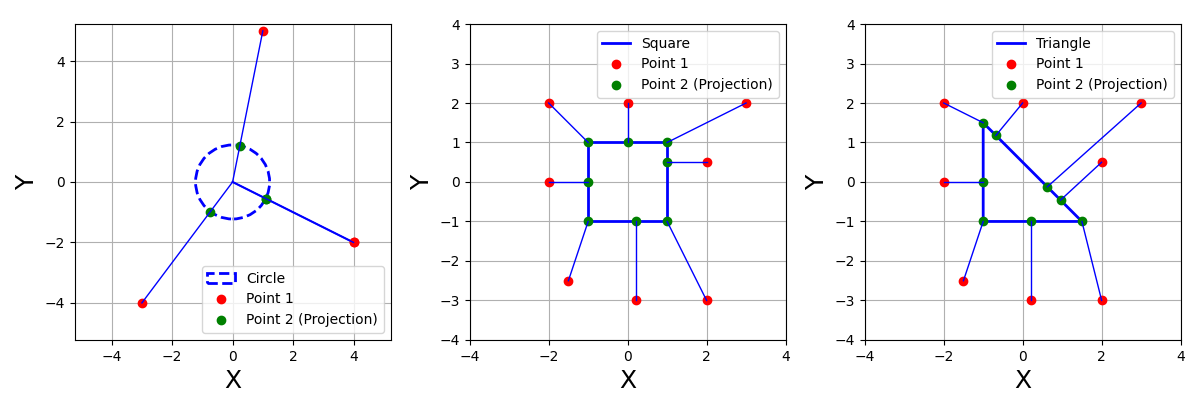
\includegraphics[width=0.99\columnwidth]{figures/projections.png}
    \caption{Closest point projection to different domains.}
    \label{fig:proj}
\end{figure}

\subsection{Using PGD on the function}
We applied the Projected Gradient Descent (PGD) method to the function:

\[
f(x,y) = x^2 + e^x + y^2 - xy
\]

with the starting point \( x_1 = (1,1) \). This function is \(\alpha\)-strongly convex, \(\beta\)-smooth, and \(L\)-Lipschitz continuous on the three domains used. The gradient of the function is given by:

\[
\nabla f = (2x + e^x - y, 2y - x)
\]

For each domain, we performed PGD using three different learning rates, denoted by \(\gamma\):

\begin{itemize}
    \item \(\gamma_1 = \frac{\| x_1 - x^* \|}{ L\sqrt{T}}\)
    \item \(\gamma_2 = \frac{1}{\beta}\)
    \item \(\gamma_3 = \frac{2}{\alpha(k+1)}\), where \(k\) is the iteration number
\end{itemize}

We conducted 10 steps of gradient descent for each combination of learning rate \(\gamma\) and domain. The final positions after these steps are presented in Table~\ref{tab:results}. 

The approximate position of the minimum is \(x^* = (-0.43, -0.22)\), and as shown in the table, the closest approach to this minimum is achieved with \(\gamma_3\) on the circular domain.

Additionally, the PGD steps for all combinations of domains and learning rates are shown in Figure~\ref{fig:PGD}. We observe that for \(\gamma_3\), the learning rate is initially too large, but it adapts and decreases with each iteration, eventually leading to the closest convergence to the minimum.


\begin{table}[H]
    \centering
    \begin{tabular}{c|c|c|c}
     & \textbf{Circle} & \textbf{Square} & \textbf{Triangle} \\
    \hline
    $\gamma_1$ & $[-0.4799,\ 0.3517]$ & $[-0.5271,\ 0.4092]$ & $[-0.5271,\ 0.4092]$ \\
    $\gamma_2$ & $[-0.3496,\ -0.0682]$ & $[-0.3484,\ -0.0602]$ & $[-0.3484,\ -0.0602]$ \\
    $\gamma_3$ & $[-0.4345,\ -0.2190]$ & $[-0.4263,\ -0.2077]$ & $[-0.4236,\ -0.2039]$ \\
    \end{tabular}
    \caption{Convergence results for circle, square, and triangle domains for different learning rates.}
    \label{tab:results}
\end{table}

    \begin{figure}[h]
        \centering
        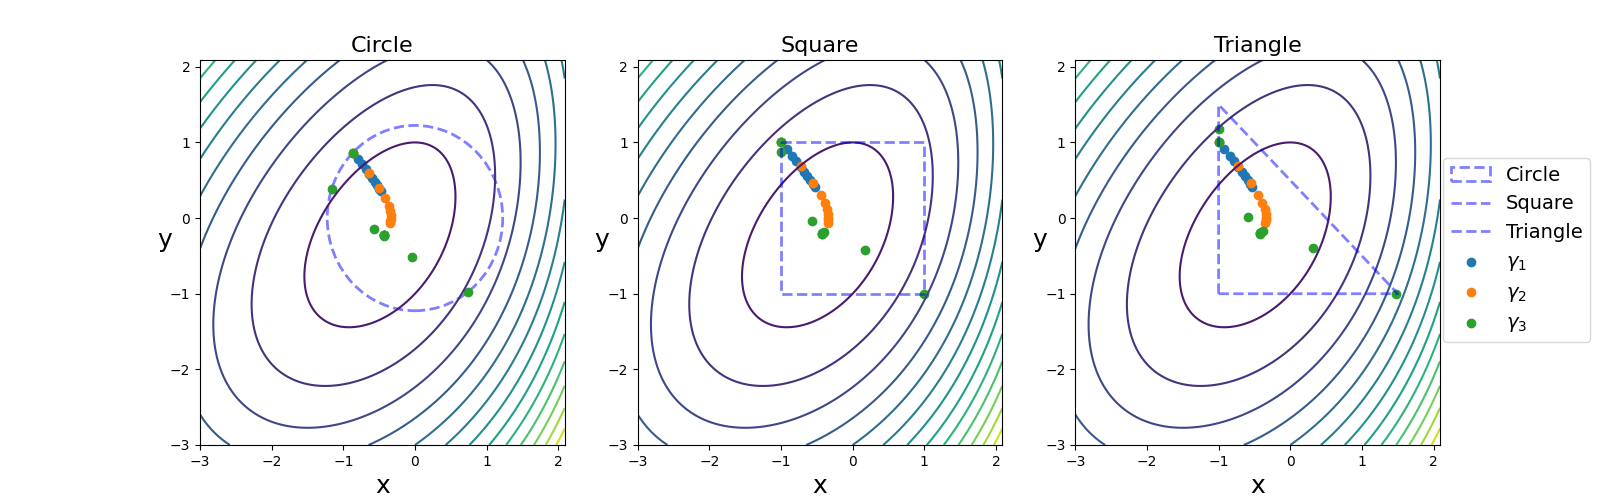
\includegraphics[width=0.99\columnwidth]{figures/PGD.png}
        \caption{PGD for different learning rates and domains}
        \label{fig:PGD}
    \end{figure}

We also checked the theoretical guarantees from Theorem 3.3 in the notes. The results are presented in Table~\ref{tab:guarantees}. As observed, all the guarantees are easily satisfied. Additionally, we note that the results do slightly vary with different domains.


\begin{table}[H]
    \centering
    \begin{tabular}{c|c|c|c}
    \textbf{Condition} & \textbf{Circle} & \textbf{Square} & \textbf{Triangle} \\
    \hline
    Cond 1 & $0.8554 \leq 6.2477$ & $1.1567 \leq 5.4298$ & $1.1567 \leq 6.2477$ \\
    Cond 2 & $0.0188 \leq 5.1256$ & $0.0206 \leq 6.7972$ & $0.0206 \leq 6.7972$ \\
    Cond 3 & $0.0188 \leq 0.7704$ & $0.0206 \leq 1.0200$ & $0.0206 \leq 1.0200$ \\
    Cond 4 & $6.49\cdot10^{-5} \leq 36.7375$ & $0.0046 \leq 36.7375$ & $0.0101 \leq 36.7375$ \\
    \end{tabular}
    \caption{Convergence guarantees for circle, square, and triangle domains.}
    \label{tab:guarantees}
    \end{table}
    
\section{Problem 6}
In this problem we tried to find the global minimum of the function:
\begin{equation}
    f(z) = - \sum_{i=1}^{4} c_i \cdot e^{-\sum_{j=1}^{3} a_{ij} (z - p_{ij})^2}
    \end{equation}
    
    
    using gradient descent. The partial derivative w.r.t. $z_k$ is calculated as follows:
    \begin{equation}
        \frac{\partial f}{\partial z_k} = 2 \sum_{i=1}^{4} c_i \cdot a_{ik} (z_k - p_{ik}) \cdot e^{-\sum_{j=1}^{3} a_{ij} (z - p_{ij})^2}
    \end{equation}
    
    The gradient is then 
    \begin{equation}
        \nabla f(z) = (z_1, z_2,z_3)
    \end{equation}
         
        When experimenting with different starting points and learning rates for gradient descent (GD), we observed that the procedure often gets stuck at local minima. This led us to believe that the function has multiple local minima. To address this, we performed a grid search over our domain, which is $[0,1]^3$. The search evaluated the function values at different points, with a step size of 0.1 (resulting in 1000 steps in total) across the three variables.

        From this grid search, we identified the point with the smallest function value, 
        located at $(0.1, 0.6, 0.9)$, as our starting point for GD descent. According to 
        the instructions in the Homework, this point was a good choice since it allowed us 
        to get quite close to the reported approximate minimum. The function values and
         corresponding positions for different learning rates are presented in Table~\ref{tab:res_6}.
         We can see that the closes result was achieved for learning rates 0.008 or lower. Note that we stopped 
         the methoed when the gradient step was less than $10^{-15}$.  


         \begin{table}[h]
            \centering
            \begin{tabular}{c|c|c|c}
                \textbf{$\gamma$} & \textbf{Iterations} & \textbf{Final Point} & \textbf{Function Value} \\
                \hline
                1        & 1      & [0.09302137, -2.096733, -8.01761408]           & -0.0 \\
                0.1      & 1      & [0.1, 0.6, 0.9]                                & -3.586922560937449 \\
                0.0102   & 2087   & [0.11461434, 0.55564885, 0.85254695]           & -3.8627821478207554 \\
                0.01     & 2128   & [0.11461434, 0.55564885, 0.85254695]           & -3.8627821478207554 \\
                0.008    & 2641   & [0.11461434, 0.55564885, 0.85254695]           & -3.862782147820755 \\
                0.005    & 4156   & [0.11461434, 0.55564885, 0.85254695]           & -3.862782147820755 \\
                0.001    & 19499  & [0.11461434, 0.55564885, 0.85254695]           & -3.862782147820755 \\
                0.0001   & 176068 & [0.11461434, 0.55564885, 0.85254695]           & -3.862782147820755 \\
            \end{tabular}
            \caption{Results for different learning rates ($\gamma$) showing the number of iterations, final point, and function value.}
            \label{tab:res_6}
        \end{table}




\end{document}
